\chapter{Theoretical Background}

\red{CHAPTER STATUS: IN PROGRESS}

The topic of this paper is the exploration of the sub-structure of the \emph{nucleon}, a particle that makes up an atom's nucleus which can be either a proton (\emph{p}) or a neutron (\emph{n}). By sub-structure, I refer to the nucleon's composition and the momentum distributions carried by the nucleon's constituent particles, quarks and gluons.

While a complete review of the history and physics behind nucleon structure and its investigative probes is beyond the scope of this paper, a brief overview of Drell-Yan, parton distribution functions, and nuclear structure phenomenology will help in understanding concepts and terminology relevant to this and later chapters.

\section{Introduction}

The first indication that the proton may have some internal structure was in a 1933 experiment by Estermann \emph{et al.} measuring the magnetic moment of the proton \cite{Estermann:169E}. Since the proton was thought to be a point-like Dirac particle, it's magnetic moment ($\mu_p$) was expected to be $\mu_p = \frac{e}{2 m_p} = 1 n.m.$, or one \emph{nuclear magneton}. The experiment resulted in a value of 2.5 n.m., leading many to reconsider the notion that the proton is indeed point-like.

Around the same time, Hideku Yukawa is credited for establishing the first theory of a \emph{strong force}, a force binding together nucleons in a nuclei against the sizable \emph{Coulomb} repulsion of protons against each other. The force was theorized to be mediated by the exchange of particles called \emph{mesons}, and its range was limited to nuclei-scale distances, seeing as it's not observed at larger distances. Based upon the size of the nucleus, Yukawa estimated the mass of the intermediating particles to be approximately $2 \times 10^2 m_e \approx 100 MeV$, where $m_e$ is the electron mass. The following year, Anderson et al. discovered the muon ($\mu$) at around this mass\CN, which confused many as it did not seem to partake in strong interactions. Eventually, by 1947, the meson theory was validated by the discovery of the \emph{pion} by Powell \emph{et al.}\CN, and Yukawa was awarded a Nobel Prize for his theory in 1949. While the pion turned out to be just another composite particle, its discovery was a watershed moment in particle physics that led to a cascading series of discoveries. 
\begin{figure}
	\centering
	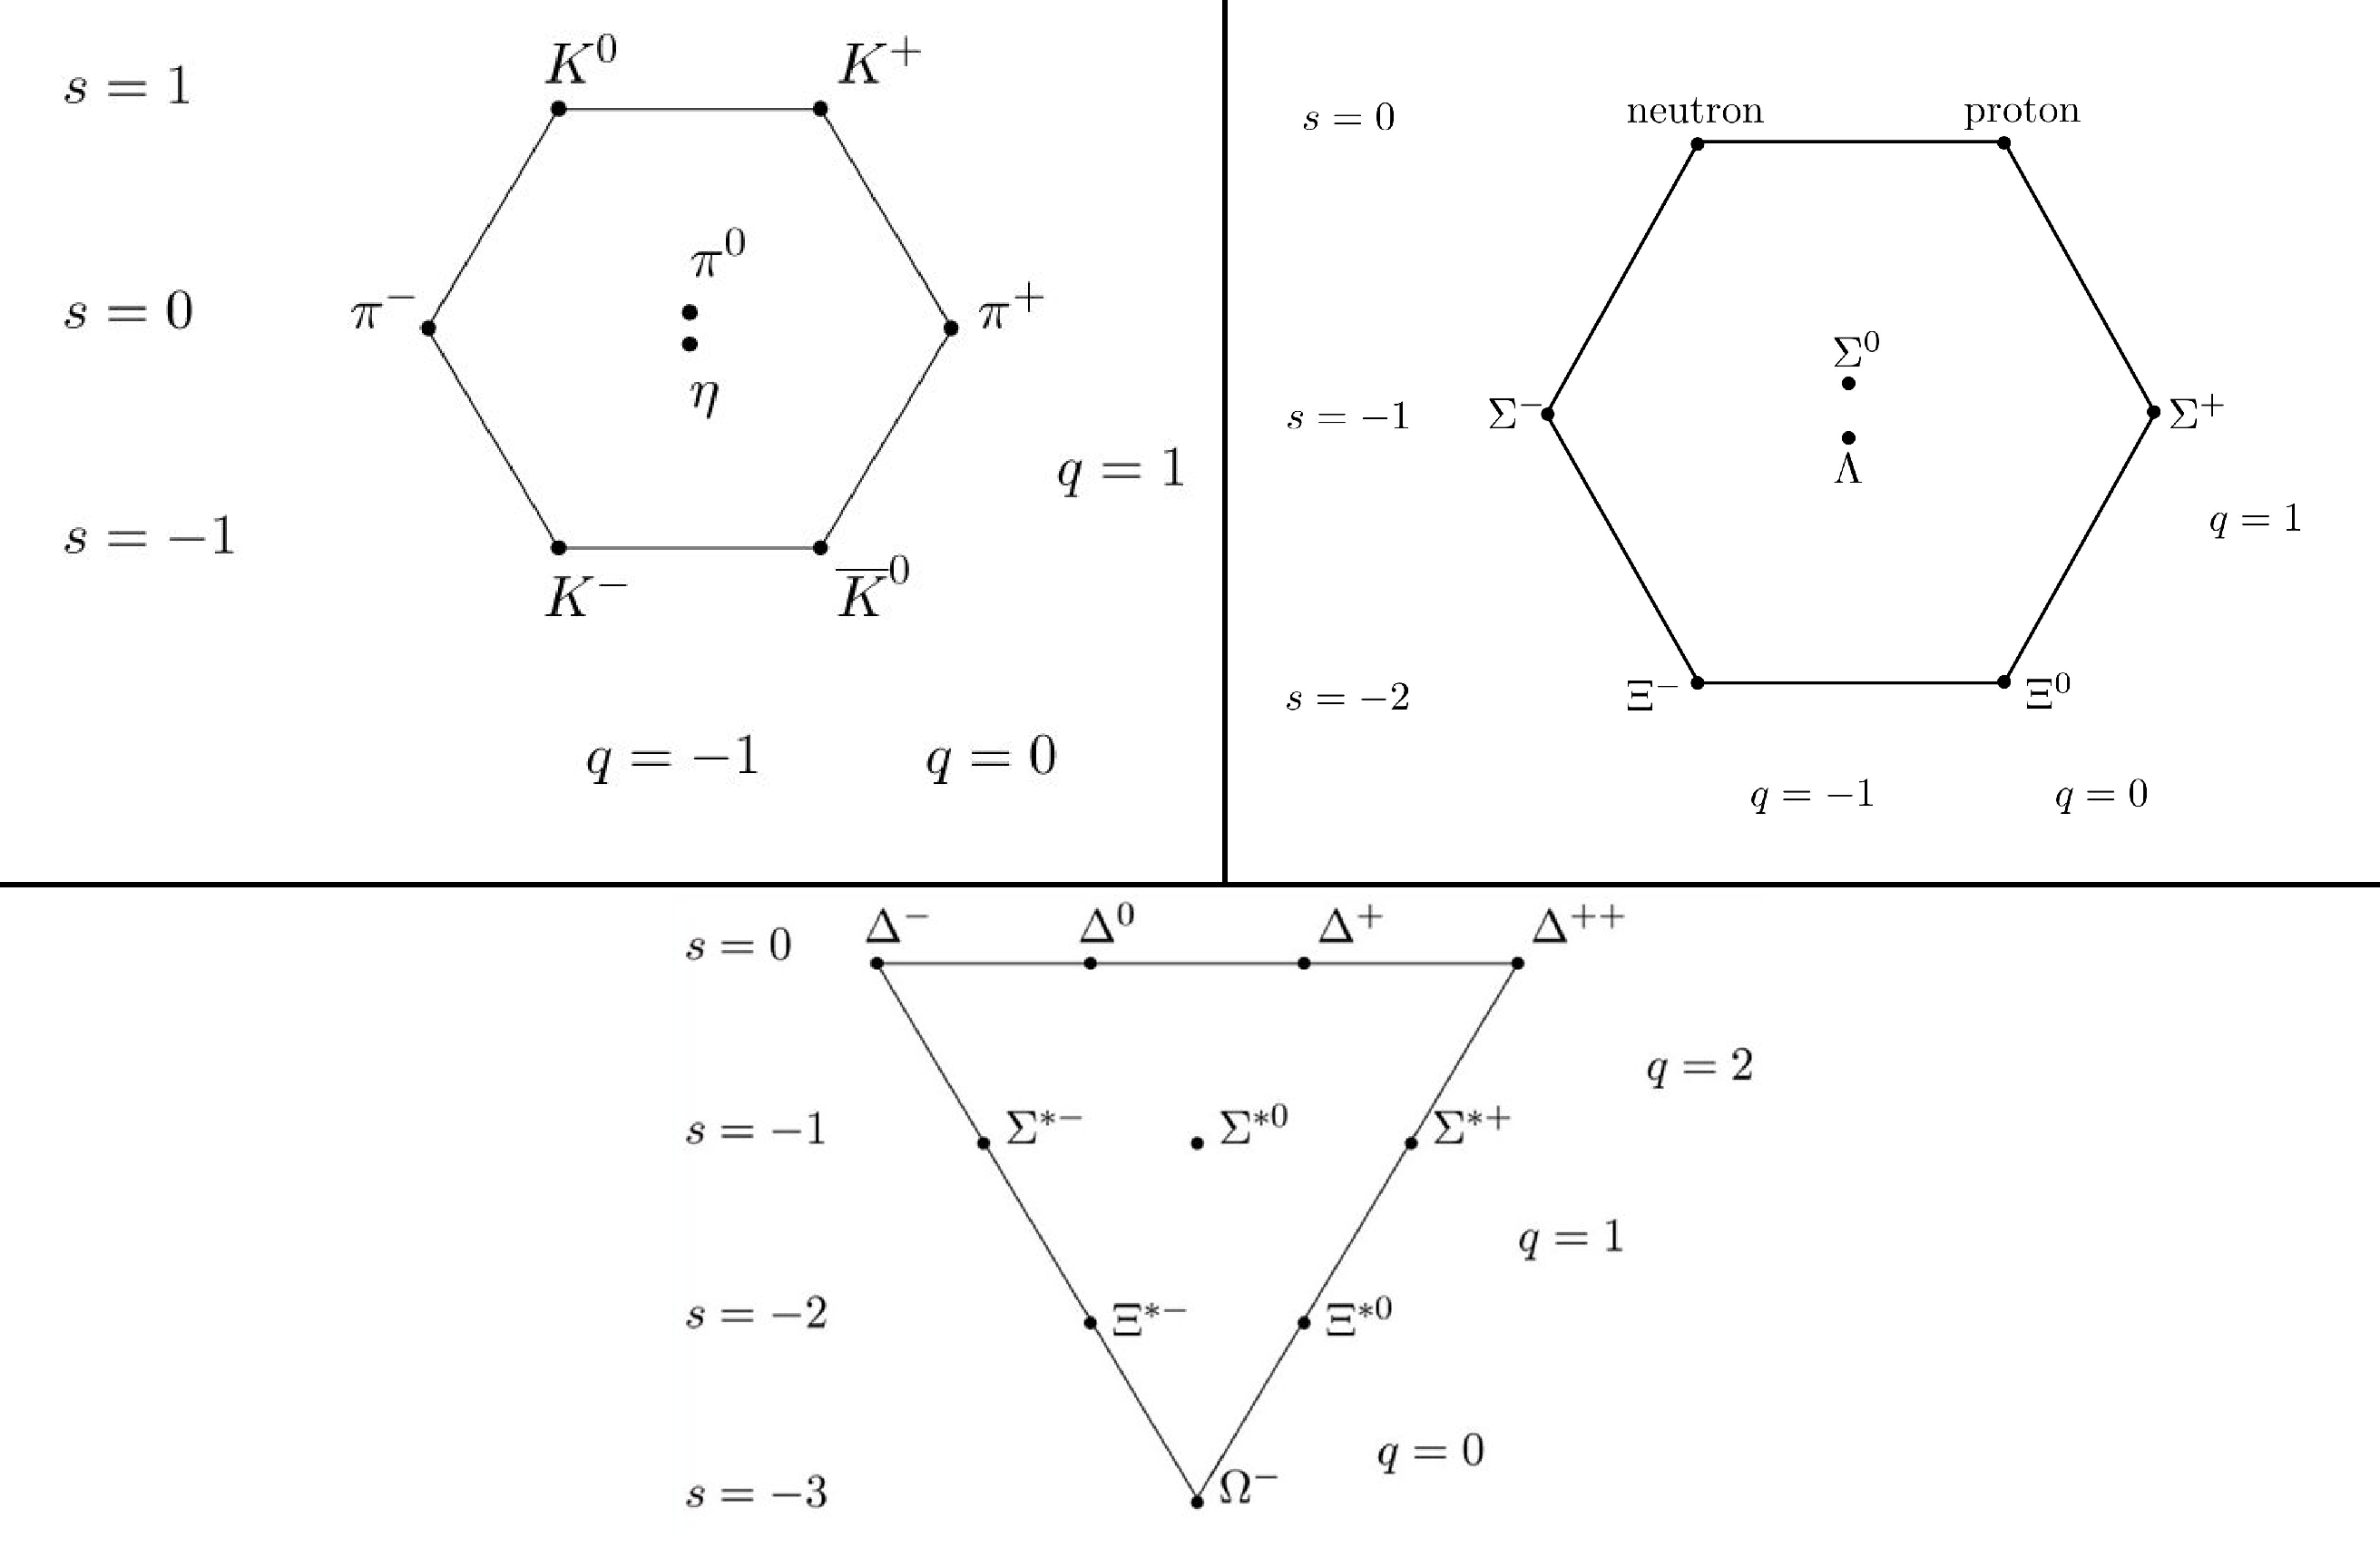
\includegraphics[width=4.5in]{figures/background/mesons_baryons.pdf}
	\caption{The octets and decuplet of Gell-Mann's ``Eightfold Way''. Top left: the eight particles of the meson octet; top right: the spin-$\frac{1}{2}$ baryon octet; bottom: the spin-$\frac{3}{2}$ baryon decuplet.}
	\label{fig:mesons-baryons}
\end{figure}

Near the end of the 1960's, SLAC began the first set of experiments to use an electron beam to investigate the nucleon in what is now known as Deep Inelastic Scattering (DIS). What they discovered was that the functions used to describe nuclear structure were largely independent of momentum transfer ($Q^2$) above a certain threshold. This so-called ``scaling'' behavior lent credence to the theory that nucleons were composed of a point-like particles. This discovery coupled with the proliferation of new particles (the ``particle zoo'') led Murray Gell-Mann and Yuval Ne'eman to construct a framework that would make some sense of it all. Gell-Mann had organized the host of mesons and baryons discovered into a geometric order named the ``Eightfold Way''\footnote{Gell-Mann here makes a rather poetic allusion to the Buddhist ``Noble Eightfold Path''} as depicted in Figure~\ref{fig:mesons-baryons}. The underlying explanation for all of this, as described independently by Gell-Man and Ne'eman, was to characterize these many particles as the several combinations of three \emph{flavors} of constituent particles, named \emph{quarks}. The flavors, \emph{u}, \emph{d}, and \emph{s} were named \emph{up}, \emph{down}, and \emph{strange}. Here, mesons were predicted to be composite particles of integer spin containing two quarks and baryons be half-integer spin particles composed of three quarks. This model led Gell-Mann to predict the existence of the $\Omega^-$ particle, along with its \emph{strangeness}, charge, and mass. The discovery of this particle\cite{1964PhRvL:12204B} earned Gell-Mann the 1969 Nobel Prize for his work on the quark model.

Though this model was a breakthrough in the understanding of fundamental particles, it did not comprehensively describe all experimental data. For example, when accounting for the total momentum of a nucleon, it was found that only $\sim50\%$ of the momentum was being carried by the quarks. It was not until the theory of quantum chromodynamics (QCD) came along that this and several other mysteries could be explained. QCD described the mechanism of a 3-fold \emph{color} charge and the gauge bosons, gluons, that intermediate the strong force between quarks (and other gluons). In the particular case of the missing momentum, this was found to reside in the intermediating gluons\cite{PhysRevLett.43.830}, which carry only color charge, to which the electro-weak probes used were insensitive.

Many nuclear probes and methods have been used to characterize the distributions and characteristics of nuclear partons, including the aforementioned DIS process. As I will describe later in this section, much has been learned about parton probability distribution functions with this and other processes, but it is the process of hadron-hadron di-lepton production that is of primary focus in this paper, which allows for an alternative approach to investigate the structure and characteristics of the quarks inside of a nucleon, and perhaps shed some light on some ongoing mysteries in nuclear physics.

\section{Di-lepton production in nucleon-nucleon collisions}

Studying the production of pairs of leptons resulting from hadron-hadron collisions has proven to be a powerful tool in probing nucleon structure and parton distribution functions (PDFs). Figure \ref{fig:DY-spectrum} shows the mass spectrum of the muon mode of di-lepton production in proton-nucleus collisions measured at the E-866/NuSea experiment at Fermilab\cite{PhysRevLett.80.3715}. The resonances of the $J/\Psi$, $\Psi^\prime$, $\Upsilon$, $\Upsilon^\prime$, and $\Upsilon^{\prime\prime}$ can be seen atop a smooth, continuous distribution which decreases with mass. The process responsible with this distribution of $\mu^+\mu^-$ pairs is the Drell-Yan process\cite{PhysRevLett.25.316}, which is illustrated in the Feynman diagram in Fig.~\ref{fig:dy-diagram}. This process is characterized by a quark annihilating with an anti-quark to form a virtual time-like photon which then decays into a pair of leptons. The study of this process can lend some insight into nucleon structure due to the fact that the mass and momentum of the di-lepton pair directly reflects the momentum distributions of the interacting quarks and anti-quarks. Current knowledge and models\CN of these momentum distributions come primarily from deep-inelastic lepton scattering (DIS) and the Drell-Yan (DY) process.

\begin{figure}
	\centering
	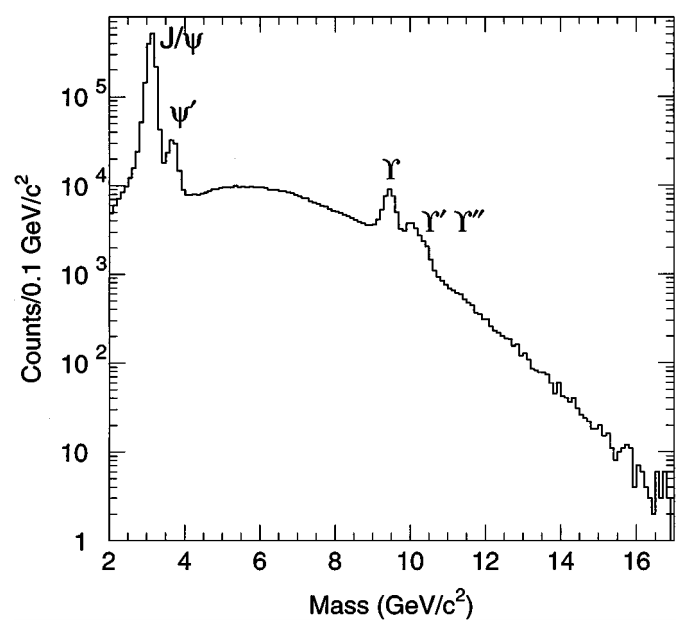
\includegraphics[width=4in]{figures/background/DY-spectrum-e866.png}
	\caption{Dimuon mass spectrum from E-866 $p+h$ collisions at \unit[800]{GeV/c}\cite{PhysRevLett.80.3715}.}
	\label{fig:DY-spectrum}
\end{figure}

%Di-lepton production has a record of being used as a technique for searching for new particles. 
One particular focus of study for the Drell-Yan process is its nucleon number-dependent (A-dependent) behavior of its cross sections. This is of particular interest due to a phenomenon known as the EMC effect, in which the European Muon Collaboration (EMC) discovered in 1983 that parton distribution functions become modified when in the presence of the nuclear medium. This A-dependent behavior was not expected for hard scattering processes as the modest (maximum $\unit[8.8]{MeV}$) binding energy of a nucleus on a nucleon was not thought to have a significant effect on quark momentum distributions within a nucleon (\unit[938]{$Mev/c^2$}). Many experiments since\CN have confirmed, extended, and precisely characterized the A-dependent behavior observed. Among the many hard scattering probes for investigating this phenomenon, the Drell-Yan process is uniquely capable of isolating the effect on the anti-quark distributions to a high degree of accuracy. The study of the effects of the nuclear medium on nucleon anti-quark distributions is the secondary research goal of the SeaQuest experiment and is the main focus of this thesis.

Within this thesis, the Drell-Yan process and its properties are discussed in \red{sections so and so} and various A-dependent behaviors seen in Drell-Yan and DIS are discussed in \red{sections so and so}. A few models are discussed in an attempt to theoretically characterize this A-dependent behavior in \red{sections so and so}.

In cases where a Drell-Yan process occurs, it can often be the case that the incident quark must pass through the strongly-interacting nuclear medium prior to its annihilation with the anti-quark in the target. By investigating the momentum distribution of the quark from the beam and it's A-dependence, some insight can be gained regarding the parton energy loss as it moves through a foreign nuclear medium. This topic and its existing data are briefly discussed in \red{section so and so}.

\subsection{The Drell-Yan Process}

\begin{figure}[h]
	\centering
	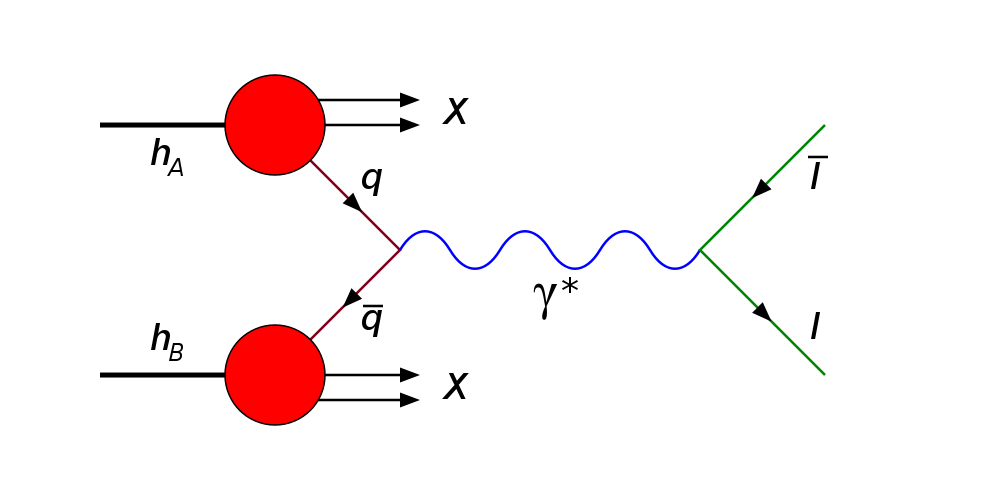
\includegraphics[width=5.0in]{figures/background/Drell-Yan.png}
	\caption{The Drell-Yan process, an $s$ channel interaction consisting of the annihilation of a quark with an anti-quark.}
	\label{fig:dy-diagram}
\end{figure}

The study of continuum di-lepton production in hadron collisions,
\begin{equation}
	h_A +  h_B \rightarrow l^+ l^- + X
	\label{eq:hh2ll}
\end{equation} 
can be used to study hadronic structure in a way that is complementary to the study of deep-inelastic scattering,
\begin{equation}
l + h \rightarrow l^\prime + X.
\label{eq:lh2lx}
\end{equation}
In 1970, S. Drell and T.M. Yan were the first to suggest that, at high $Q^2 (=M^2_{l^+ l^-}) \geq 16GeV^2$, the quarks inside the hadrons $h_A$ and $h_B$ can be considered free fermions in the instantaneous moment that they interact. The Drell-Yan model addresses the dominant subprocess here,
\begin{equation}
q_A + \bar{q}_B \rightarrow \gamma^* \rightarrow l^+ l^-
\label{eq:dy-process}
\end{equation} 
as an electromagnetic annihilation process. In this high-$Q^2$ kinematic space, the final state of the hadrons that contain these quarks becomes more or less irrelevant. By the energy-time uncertainty principle\CN of $\Delta E \Delta t \sim \hbar$, the timescales under consideration are $<10^{-25}s$, and the corresponding distances are $<10^{-17}m$, where the size of a nucleon is $\sim 10^{-15}m$\CN. At these short space-time scales, electromagnetic annihilation dominates this quark-quark interaction.

This is further reinforced by the widely accepted non-Abelian gauge field theory of Quantum Chromodynamics (QCD) which describes the interactions between quarks and gluons. QCD provides a theoretical justification for treating Drell-Yan processes as events isolated from the rest of the hadron states, and it does so through the concept of the running of the coupling constant, or \emph{asymptotic freedom}\cite{Bethke:2006ac}. This characteristic feature of QCD is described by the decrease of the strength of the strong force coupling constant as the space-time scale of the interaction approaches zero (i.e. as $Q^2 \rightarrow \infty$). The strong coupling constant can be expressed as a function of $Q^2$:
\begin{equation}
\alpha_s(Q^2) = \frac{1}{\beta_0 \ln (Q^2/\Lambda^2)}
\end{equation}
where
\begin{equation}
\beta_0 = \frac{12\pi}{33-n_f}
\end{equation}
Here, $\Lambda$ is the QCD scale parameter that depends on the number of quark flavors, $n_f$, and the renormalization scheme, measured to be around $\sim$ \unit[217]{MeV}. Experimental measurements of the running of the coupling constant as measured by many different processes can be seen in Figure~\ref{fig:asymptotic-freedom}.
\begin{figure}
	\centering
	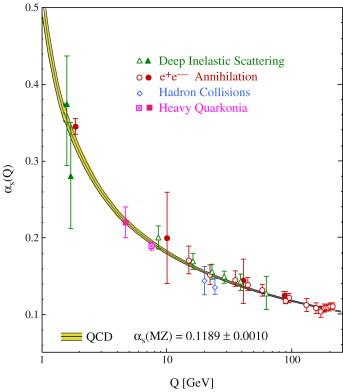
\includegraphics[height=2.5in]{figures/background/asymptotic-freedom.jpg}
	\caption{A compilation of measurements of the running of the strong coupling constant, $\alpha_s(Q^2)$.}
	\label{fig:asymptotic-freedom}
\end{figure}

\subsection{Drell-Yan Kinematics}

In the center-of-mass frame, the Drell-Yan process can be broken down into three stages with three sets of kinematics (refer to Fig.~\ref{fig:dy-diagram}). Beginning with the quarks, \emph{x} is defined as the fraction of the hadron's momentum carried by the interacting quark or antiquark. Conventionally in fixed-target experiments, subscripts are assigned as $x_1$ and $x_2$, which refer to the quark/antiquark from the beam and the antiquark/quark from the target, respectively. This \emph{x} is called the Bjorken \emph{x}, and is well-known in DIS processes to have a value of
\begin{equation}
x = -q^2/2 p \cdot q
\end{equation} where \emph{p} and \emph{q} are the 4-momenta of the hadron and the photon.

The next stage of the process is the virtual photon. This photon' properties are effectively equivalent to the `dimuon' or `dilepton', which are the terms more commonly used in referring to kinematics. The first of its relevant kinematics is its mass $M_{\gamma^*}$, which represents its energy and virtuality. The value $x_F$, or Feynman-x, is the fraction of the maximum possible longitudinal momentum carried by the virtual photon in the beam direction. The transverse momentum, $p_T$, and the azimuthal production angle, $\phi_{\gamma^*}$ are the remaining kinematics associated with the virtual photon.

The third stage regards the pair of leptons produced. In the frame of the virtual photon, there is a polar and azimuthal decay angle, $\theta_\mu$ and $\phi_\mu$, respectively, for each of the decay muons. It becomes impossible, however, to reconstruct these variables, as the individual transverse momenta of the quarks are unknown, and the thus the quark-antiquark annihilation axis is unknown. This is remedied by shifting the process into the Collins-Soper (CS) reference frame\cite{PhysRevD.16.2219} which orients the reference axis to be parallel to the bisector of the angle between the interacting hadrons in the rest frame of the muon pair. A depiction of the Collins-Soper frame can be found in Fig.~\ref{fig:collins-soper}. In total, this brings a total of eight kinematic variables, summarized in Table~\ref{tab:var}.
\begin{figure}
	\centering
	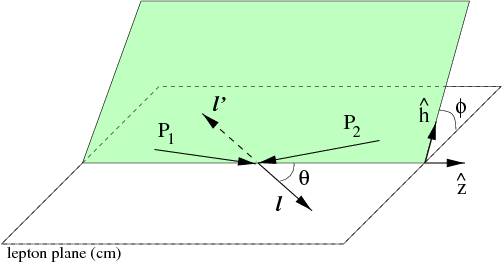
\includegraphics[width=4.50in]{figures/background/collins-soper.png}
	\caption{A depiction of the Collins-Soper reference frame. The green plane along $\hat{h}$ is the plane shared by the two hadrons.}
	\label{fig:collins-soper}
\end{figure}

Experimentally, six independent variables are measured, which form a basis by which all eight can be known. This is due to the fact that two pairs of variables, ($M_{\gamma^*}$, $x_F$) and ($x_1$, $x_2$) are correlated by the following, ignoring quark masses and considering $p_\perp << p_{\ell}$:
\begin{eqnarray}
x_F & \equiv & \frac{p_{\ell}}{\sqrt{s}/2} \approx x_1 - x_2 \label{eq:xf=x1-x2} \\
M_{\gamma^*}^2 & \equiv & E^2 - p_{\ell}^2  = s x_1 x_2 \label{eq:m=sx1x2} \\
E & = & \frac{1}{2}(x_1 + x_2) \sqrt{s} \\
p_{\ell} & = & \frac{1}{2}(x_1 - x_2)\sqrt{s}
\end{eqnarray}
In this frame, the longitudinal momenta of the quarks are $x_1 \sqrt{s}/2$ and $- x_2 \sqrt{s}/2$, with $\sqrt{s}$ being the center of mass energy of the hadronic collision. So, by measuring the 3-momenta of the $\mu^+$ and $\mu^-$, the quantities ($M_{\gamma^*}$, $x_F$, $p_T$, $\phi_{\gamma^*}$, $\theta_\mu$, $\phi_\mu$), which is sufficient to calculate the remaining ($x_1, x_2$) in our approximation.

\begin{table}[h]
	\centering
	\begin{tabular}{c|r}
		Variable&Description\\ \hline \hline
		$x_{1/2}$ & Momentum fraction of the beam/target quark\\
		$M_{\gamma^*}$ & Mass of the virtual photon (dimuon)\\
		$x_F$ & Fraction of the max. possible $p_{\ell}$ carried by virt. photon\\
		$p_T$ & Transverse momentum carried by the virt. photon\\
		$\theta_{\mu}, \phi_{\mu}$ & Polar and azimuthal decay angle\\ & of one of the muons, in the CS ref. frame\\ \hline
		$\alpha$ & The fine structure constant \\
		$K(x_1,x_2)$ & High-order QCD correction term \\
		$\sqrt{s}$ & Center of mass energy of the hadronic collision \\
		$\sqrt{\hat{s}}$ & Center of mass energy of the $q\bar{q}$ collision \\
		$Q^{2}$ & Four-momentum of the intermediate time-like photon, squared \\ 
		$q_i^{t/b}(x)$ & The quark number density in the nucleon of the target/beam \\ \hline \hline
	\end{tabular}
	\caption{Kinematic variables relevant to the Drell-Yan process .}
	\label{tab:var}
\end{table}

\subsection{Cross-Section}

As the participating quarks are asymptotically free within each hadron, there will be no correlations between the probability distributions of the annihilating particles, and the process is independent of the distributions. As a result, the cross section of the Drell-Yan process can be reduced to a function of the electromagnetic annihilation process and the quark probability distribution functions. With these components and some QCD considerations, we can construct it piece by piece.

The first step is to begin with the known hard scattering cross section of $\epsilon + \bar{\epsilon} \rightarrow l^+ l^-$, where $\epsilon$ is an arbitrary particle. This cross section\cite{Halzen:1984mc} is given by
\begin{equation}
\sigma(\epsilon\bar{\epsilon}\rightarrow l^+l^-) = \frac{4 \pi \alpha^2}{3M_{\gamma^*}^2} e_f^2
\label{eq:annihilation-cross}
\end{equation}
where $\alpha$ is the electromagnetic fine structure constant, $e_f$ is the charge of the particle, and $M_{\gamma^*}$ is the dilepton mass. With this, we add the QCD consideration that only $q\bar{q}$ of opposite color can annihilate with each other into a colorless virtual photon. Possible combinations are $R\bar{R}$, $B\bar{B}$, and $G\bar{G}$ out of $3\times 3$ possible cases. As such, an overall factor of $\frac{1}{3}$ is added to this cross section. Finally, factoring in the conservation of flavor (there can only be $u\bar{u}$, $d\bar{d}$, etc. combinations) and the quark structure of hadrons A and B,  we use the product ($q_f^A(x_1)\bar{q}_{f}^B(x_2)$) of the quark probability distributions for finding quarks of the same flavor-antiflavor combination in the two hadrons. It must also be considered that the quark or antiquark may be found in either hadron A or hadron B. The product of these three factors leads us to the Drell-Yan cross section\cite{Drell:1970wh}
\begin{eqnarray}
\frac{d^2\sigma}{dx_1dx_2}&=&\frac{1}{3}\frac{4\pi\alpha^2}{3M_{\gamma^*}^2}
\sum_{f}e_f^2[q_f^A(x_1)\bar{q}_f^B(x_2)+
\bar{q}_f^A(x_1)q_f^B(x_2)]\\
&=&\frac{4\pi\alpha^2}{9 s x_1 x_2}
\sum_{f}e_f^2[q_f^A(x_1)\bar{q}_f^B(x_2)+
\bar{q}_f^A(x_1)q_f^B(x_2)]
\label{eq:DY-cross}
\end{eqnarray}
where the sum is summing over flavors of quarks ($f\in\{u,d,s,...\}$). This can be evaluated in terms of the measurables $M_{\gamma^*}$ and $x_F$ via Equations~\ref{eq:xf=x1-x2}~and~\ref{eq:m=sx1x2}
\begin{equation}
M_{\gamma^*}^2 \frac{d^2\sigma}{dM_{\gamma^*}^2 dx_F} = 
\frac{1}{3}\frac{4\pi\alpha^2}{3M_{\gamma^*}^2}
\frac{x_1 x_2}{x_1 + x_2}
\sum_{f}e_f^2[q_f^A(x_1)\bar{q}_f^B(x_2)+
\bar{q}_f^A(x_1)q_f^B(x_2)]
\label{eq:dy-cs-observe}
\end{equation}
where $x_1$ and $x_2$ can be expressed as
\begin{equation}
x_1 = \frac{1}{2}\left[\sqrt{x_F^2 + 4\tau} + x_F\right],\ \  
x_2 = \frac{1}{2}\left[\sqrt{x_F^2 + 4\tau} - x_F\right],\ \ 
\tau = \frac{M_{\gamma^*}^2}{s}
\end{equation}
The cross section can also be represented by dimensionless variables in its scaling form,
\begin{equation}
s \frac{d^2\sigma}{d \sqrt{\tau} dy} = 
\frac{1}{3}\frac{4\pi\alpha^2}{3}
\sum_{f}e_f^2[q_f^A(x_1)\bar{q}_f^B(x_2)+
\bar{q}_f^A(x_1)q_f^B(x_2)]
\label{eq:dy-cs-dimensionless}
\end{equation}
where we introduce the rapidity term $y$ in describing $x_1$ and $x_2$,
\begin{equation}
y  = \frac{1}{2} \ln \frac{E+ p_\ell}{E-p_\ell} = \frac{1}{2} \ln \frac{x_1}{x_2},\ \ 
x_1  = \sqrt{\tau} e^{y},\ \  
x_2  = \sqrt{\tau} e^{-y}
\end{equation}
It should be noted that with collider experiments, it is conventional to refer to the hadrons A and B in terms of the beam and target hadrons, respectively, and as such, $x_1$ refers to the the quark in the beam hadron and $x_2$ refers to the quark in the target hadron.

In each of these equations~\ref{eq:DY-cross}, \ref{eq:dy-cs-observe}, and \ref{eq:dy-cs-dimensionless}, the cross sections can be factored into two parts: one subprocess cross section and one part that has only a dependence on the parton distribution functions. They are independent of each other, because one of the staples of the quark parton model is that the PDFs ($q(x) and \bar{q}(x)$) are independent of the process by which they are probed. At this point, let's look a bit more deeply into these PDFs, how they're measured, and their behavior.

\subsection{The Quark Parton Model and PDFs}

%Let's say that we have two hadrons A and B colliding; a parton of type \emph{a} ($u, d, s, g$, etc.) comes from A and carries with it a fraction of A's momentum ($x_A$).  The same goes for hadron B; a parton of type \emph{b} comes from B and carries momentum fraction $x_B$. Now, the probability of finding the discussed parton from A is given by $f_{a/A}(x_A)dx_A$. Likewise, the probability of finding the discussed parton from B is $f_{b/B}(x_B)dx_B$.  
%
%These \emph{structure functions}, $f_{a/A}(x)$ are called the \emph{parton distribution functions} (PDF's), and they have been the focus of a great deal of experiments over the years by several collaborations. Due to the complex nature of lattice QCD, these PDF's are determined empirically, with only a few rules based in theory. It is important to note that there is normally a $Q^2$ dependence of these PDF's. At high enough $Q^2$, as it is in the case of our experiment, the PDF's no longer scale with $Q^2$ \cite{Seely:2009gt}.  That is, for a given \emph{x}, the PDF is independent of $Q^2$.
%
%An important metric to observe is the probability that a parton \emph{a} carries a momentum fraction $x_A$ in its hadron $A$.  This can be represented by the following expression: $x_A f_{a/A}(x_A)dx_A$. For Drell-Yan interactions in the study proposed here, we are interested in the momentum distribution amongst the quarks in the proton.  The CTEQ collaboration has collected data from many experiments, yielding the model represented in Figure \ref{fig:pdf} \cite{Pumplin:2002vw}.
%
%\begin{figure}
%	\centering
%	\subfloat[][The parton distribution function describing the momentum carried by different types of quark in the proton.]{%
%		\label{fig:pdf}%
%		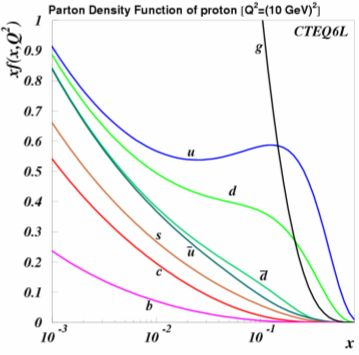
\includegraphics[width=0.40\linewidth]{figures/background/parton-dist.jpg}}%
%	\hspace{8pt}%
%	\subfloat[][The ratio of cross sections (per nucleon) as a function of the target's fractional momentum, $x_2$.  The EMC Effect region, $0.3<x_2<0.6$ is the phenomenon discussed here.]{%
%		\label{fig:emc}%
%		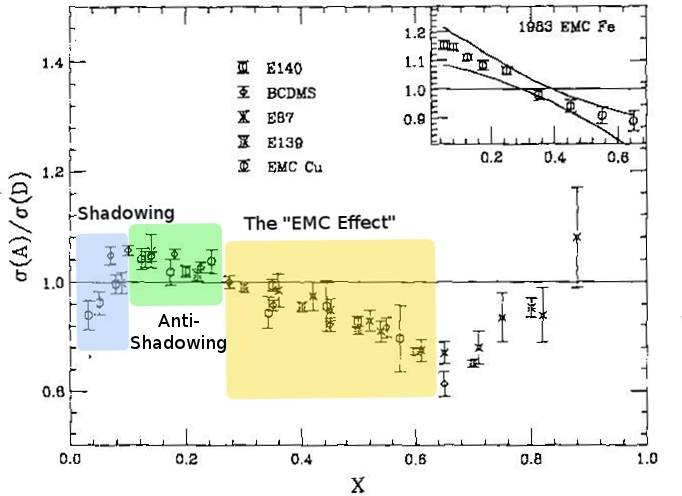
\includegraphics[width=0.53\linewidth]{figures/background/EMC_EMC.jpeg}}
%	\caption{The proton's momentum distribution and the EMC Effect, with key regions highlighted.}
%	\label{fig:pdf_emc}
%\end{figure}
%
%Looking to Figure \ref{fig:pdf} we see that at $x>0.1$, $u$ and $d$ quarks dominate $\bar{u}$ and $\bar{d}$ quarks.  This is key, because this means that, for SeaQuest where we have high $x_1$ and lower $x_2$, the Drell-Yan process is probabilistically dominated by a quark from the beam annihilating with an antiquark from the target. All antiquarks that exist in the target nucleons must come from what are called the \emph{sea quarks}, or the virtual $q\bar{q}$ pairs that pop in and out of existence amongst the gluons and valence quarks. 
%
%As we will discuss in the next section, partons in a bound nucleon behave differently than partons in a free nucleon. By studying Drell-Yan in nuclear targets, we can investigate the degree to which this modification is the result of a modification to the quark sea.
%

\subsection{QCD-Improved Drell-Yan and the K-Factor}

%In addition to the leading-order DY term, there are high-order QCD corrections to consider. These have been studied and accounted for up to $\bigoh(\alpha_s)$ and $\bigoh(\alpha_s^2)$. These include contributions from high-order $q\bar{q}$ annihilation $(q \bar{q} \rightarrow \gamma * + g)$ and gluon Compton scattering $(q + g \rightarrow \gamma * + q)$ as seen in Figure \ref{fig:nlo-dy} \cite{duan-2007-50}. The cumulative effect is denoted in the cross section as the $K(x_1,x_2)$ factor, which can vary between 1.6 and 2.8.  For our $x_1$ and $x_2$ range, $K \sim 1.6$.

\begin{figure}[h]
	\centering
	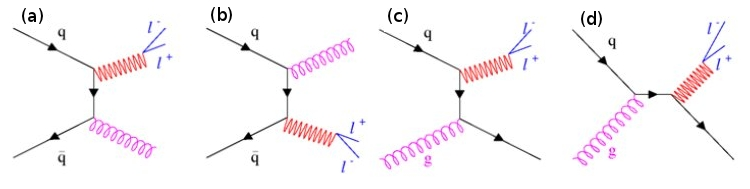
\includegraphics[width=5.00in]{figures/background/DY.jpeg}
	\caption{The Drell-Yan process has a large range of higher-order QCD corrections that need to be accounted for. 
		(A) and (B) are high order $q\bar{q}$ annihilations, and (C) and (D) are gluon ``Compton scattering'' terms.}
	\label{fig:nlo-dy}
\end{figure}

\section{Drell-Yan in Nuclei}

\subsection{The EMC Effect}

%The European Muon Collaboration, in 1983, measured the DIS cross section per nucleon ratios of $Fe$ to $D$ over a large kinematic range.  The result, as seen in the top right of Figure \ref{fig:emc} came as quite a surprise.  It was revealed that the structure function of a nucleon bound in a nucleus differs fundamentally from that of a free nucleon  \cite{Aubert:1983xm}.  This difference was not a simple or small effect either; the cross section per nucleon of a nucleus showed to be smaller than that of deuterium at very low $x_2$, greater than deuterium at $0.1<x_2<0.2$, and then steadily less than deuterium for $0.2<x_2<0.6$. 
%
%This complex, unexplained behavior opened up a new field of research and theoretical work. Following suit, the different aspects of this nuclear modification garnered some common nicknames.  The region where $x_2<0.1$ became known as \emph{``Nuclear Shadowing''}, the transition region of $0.1<x_2<0.2$ is known as \emph{"Anti-shadowing"}, and the linear decline in the ratio of cross sections between $0.2<x_2<0.6$ is generally referred to as the \emph{"EMC Effect"} \cite{Geesaman:1995yd}.
%
%The phenomenon was simple -- DIS off of a bound nucleon was not the same as off of a free nucleon -- but hundreds of theoretical papers were written attempting to explain it away, from multiquark ($6q$) clusters to the exchange of virtual pions in the nucleus. Some have joked that EMC should stand for \emph{"Every Model is Cool"}. The focus of recent work (and this paper) is on the ``EMC Effect'' region, characterized by the distinctly linear downward slope.
%
%Recent experiments at Hall C at JLab and SLAC suggest the following regarding the EMC Effect \cite{Seely:2009gt}:
%\begin{itemize}
%	\item
%	It is $Q^2$-independent
%	\item
%	It's x-dependent shape is universal (across various nuclei)
%	\item
%	The magnitude (slope) of the effect varies with A
%	\item
%	It thereby might be related to nuclear density
%\end{itemize}
%
%In parallel to this effort, many researchers were working on high-momentum nucleons and short range correlations (SRC's), neither aware yet of their common ground.

\subsection{Models For the EMC Effect}

\subsubsection{Pion Cloud Model}

\subsubsection{Nuclei-Nuclei Short Range Correlations}

\subsection{E-772 at Fermilab}
